\documentclass[12pt]{article}
\usepackage{graphicx,float,caption}
\begin{document}
	
\section{Teamwork planning}

The distribution of work and the rough timeline is presented in Table \ref{teamwork} and Figure \ref{timeline}.

\begin{table}[H]
	\centering
	\begin{tabular}{ |c|c|c| }
		\hline
		                 & \textbf{Design and implementation} & \textbf{Testing} \\ \hline
		\textbf{Ieva}    &           Names, Parser            &   GUI, Scanner   \\ \hline
		\textbf{Arsalan} &          Scanner, Parser           &    GUI, Names    \\ \hline
		\textbf{Mark}    &                GUI                 &      Parser      \\ \hline
	\end{tabular}
	\captionsetup{justification=centering,labelfont=it,textfont=it,margin=1cm}
	\caption{Work distribution among the team members}
	\label{teamwork}
\end{table}

\begin{figure}[H]
	\centering
	\captionsetup{justification=centering,margin=2cm}
	\makebox[\textwidth][c]{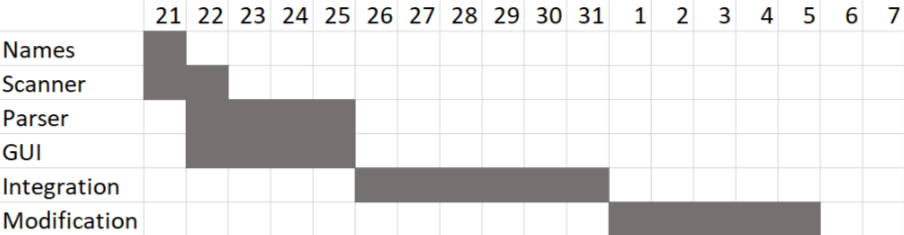
\includegraphics[scale=1]{timeline}}
	\caption{Rough timeline of the project}
	\label{timeline}
\end{figure}




\section{Errors}
\subsection{Semantic errors list}
\begin{enumerate}
	\setlength{\itemsep}{1pt}
	\setlength{\parskip}{0pt}
	\setlength{\parsep}{0pt}
	
	\item {Device with such name already exists;}
	\item {Specified device requires $[n]$ connected inputs, $[i]$ connected right now;}
	\item {DTYPE requires 4 connected inputs, $[i]$ connected right now;}
	\item {XRO requires 2 connected inputs, $[i]$ connected right now;}
	\item {Connection on the left must be an output;}
	\item {Connection on the right must be an input;}
	\item {Input/output with such name doesn't exist;}
	\item {Device with such name doesn't exist.}
\end{enumerate}
	
\subsection{Semantic error detection}
Semantic errors relating to device, input and output names will be detected by checking name tables. Whether a connection is an output or an input will also be checked using name tables and the information saved about the specific device. The number of connected inputs will be tracked as the network is built and after parsing of \textit{Connections} section is done, the number of connected inputs will be compared with device specifications.

\subsection{Error handling and reporting}

Once an error in the definition file has been detected, an error message will be printed out and a recovery will be attempted by skipping until next comma or semicolon. Building of a network will be stopped after the first error but parsing will continue in order to detect and report all errors. An example error message is given below. After parsing of the file is finished, the total number of errors will be displayed as well.

\begin{verbatim}
Line 3: CLICK CLK1 5,
        ^
Error 12: Not valid device type. Valid devices: CLOCK, SWITCH,
NAND, AND, OR, NOR, DTYPE, XOR.
\end{verbatim}


\end{document}